\section{Auswertung von Halbleiter Experiment}
Im Versuchsteil 3 wurden die Energiespektren von $^{241}$Am und $^{57}$Co mit zwei unterschiedlichen Detektoren aufgenommen. Für die Auswertung wurden hier der $122.06\,$keV so wie der $136.47\,$keV Photopeak von Cobalt so wie der $59.5\,$keV Peak von Americium mit einer Gaußkurve wie in Gleichung \ref{Gaus} gefittet. Die Peaks so wie die dazugehörigen Anpassungen für $^{57}$Co sind in Abbildung \ref{CoS} und \ref{CoC} zu sehen. Die für Americium sind in Abbildung \ref{AmS} und \ref{AmC} zu finden. Die gesamten Spektren sind im Anhang.\par
\begin{figure}[ht]
	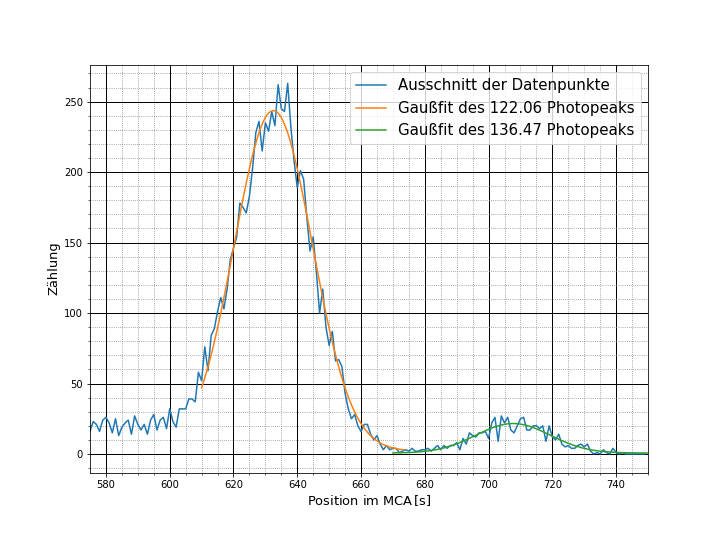
\includegraphics[scale=0.5]{Bild/CS.png}
	\centering
	\caption[V3 $122.06\,$keV und $136.47\,$keV Peaks mit Silizium Detektor]{Gaußfit für einen denn Datenbereich der $122.06\,$keV und $136.47\,$keV Photopeaks mit dem Silizium Detektor.}
	\label{CoS}
\end{figure}
\begin{figure}[ht]
	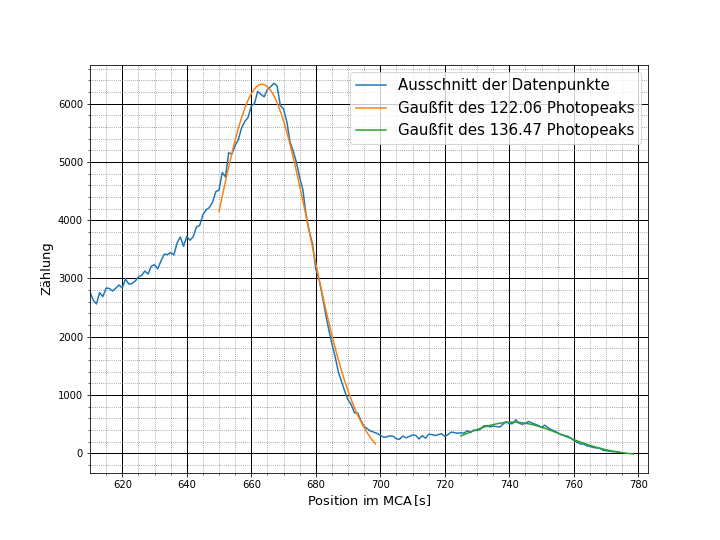
\includegraphics[scale=0.5]{Bild/CC.png}
	\centering
	\caption[V3 $122.06\,$keV und $136.47\,$keV Peaks mit CdTe Detektor]{Gaußfit für einen denn Datenbereich der $122.06\,$keV und $136.47\,$keV Photopeaks mit dem CdTe Detektor.}
	\label{CoC}
\end{figure}
\begin{figure}[ht]
	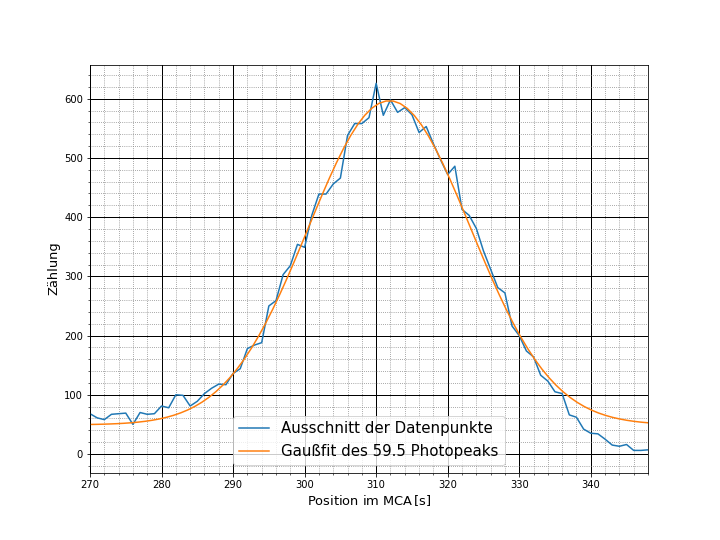
\includegraphics[scale=0.5]{Bild/AS.png}
	\centering
	\caption[V3 $59.5$\,keV Peaks mit Silizium Detektor]{Gaußfit für einen denn Datenbereich der $59.5$\,keV Photopeaks mit dem Silizium Detektor.}
	\label{AmS}
\end{figure}
\begin{figure}[ht]
	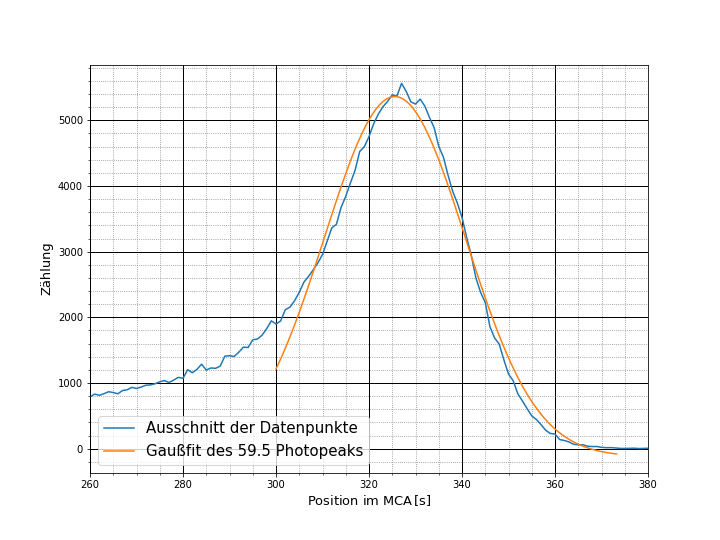
\includegraphics[scale=0.5]{Bild/AC.png}
	\centering
	\caption[V3 $59.5$\,keV Peaks mit CdTe Detektor]{Gaußfit für einen denn Datenbereich der $59.5$\,keV Photopeaks mit dem CdTe Detektor.}
	\label{AmC}
\end{figure}
\FloatBarrier
Die Position der Peaks welche die Kanalnummer des MCA's ist kann nun mit Hilfe der bekannten Energien geeicht werden, indem man separat für beide Detektoren Energie gegen Position aufträgt und die Werte dann linear anpasst. Hierbei wurde ein gewichteter Fit verwendet welche die Fehler auf die Position der Peaks berücksichtigte. Die Werte so wie die angepasste Kurve sind in Abbildung \ref{Eichung} zu sehen. Die erhaltenen Gleichungen für denn Zusammenhang zwischen Kanal und Energie sind:\par
\begin{equation*}
	f(E)_{Kanal} = (5.3988\pm 0.0010)\,\frac{1}{\text{keV}}E+(4.33\pm 0.10)
\end{equation*}
\begin{equation*}
f(E)_{Kanal} = (5.128\pm 0.008)\,\frac{1}{\text{keV}}E+(6.7\pm 0.8)
\end{equation*}
\begin{figure}[ht]
	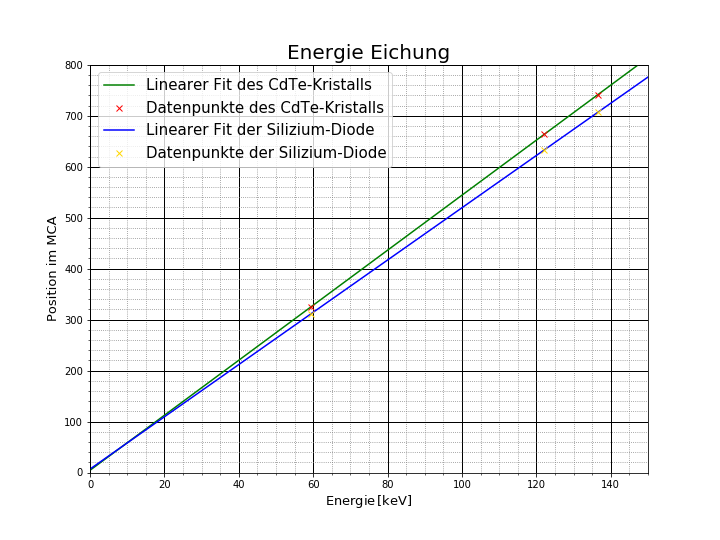
\includegraphics[scale=0.5]{Bild/Eichung.png}
	\centering
	\caption[Eichung für beide Detektoren]{Geraden zur Eichung der beiden Detektoren. In blau die Eichung für den Silizium Detektor und in grün für den CdTe Detektor. Fehler sind nicht mit eingezeichnet da sie zu klein waren um sie sinnvoll darzustellen.}
	\label{Eichung}
\end{figure}
Nun wird mit das Absorptionsverhältnis der beiden Detektoren bei unterschiedlichen Energien bestimmt. Dafür müssen die aus den Fit bestimmten Amplituden erst einmal aktive Fläche normiert werden und dann durcheinander geteilt wie in Gleichung \ref{Abs} dargestellt:
\begin{eqnarray}
\frac{Abs_{\text{Si}}}{Abs_{\text{CdTe}}}=\frac{\nicefrac{A_{\text{Si}}}{a_{\text{Si}}}}{\nicefrac{A_{\text{CdTe}}}{a_{\text{CdTe}}}}
\label{Abs}
\end{eqnarray}
Die Fläche des CdTe Detektors beträgt $a_\text{CdTe}=23\,\text{mm}^2$ und die des Si Detektors $a_{\text{Si}}=100\,\text{mm}^2$. Die erhaltenen Werte sind zusammen mit den Literaturwerten aus der Anleitung\cite{anleitung} in Tabelle \ref{MesswerteV3_1} zu finden.
Als letztes wird die Relative Energieauflösung der einzelnen Peaks bestimmt. Zur Berechnung wird die Halbwertsbreite verwendet wodurch sich folgende Gleichung ergibt:
\begin{equation}
	RER(E)=\frac{FWHM}{E}\approx\frac{2.35\sigma(E)}{E}
\end{equation}
Die erhaltenen Werte sind in Tabelle \ref{MesswerteV3_2} zu finden.
\begin{table}[ht]
	\begin{Dtabular}[1.1]{|c|c|c|}
		\hline
		Photopeak Energie [keV]&Berechnete Werte [\%] &Literaturwerte [\%]\\
		\hline
		$59.5$&$1.28 \pm 0.07$&$1,40$\\
		\hline
		$122.06$&$0.58 \pm 0.05$&$1,83$\\
		\hline
		$136.47$&$0.45 \pm 0.06$&$2,00$\\
		\hline
	\end{Dtabular}
	\centering
	\caption{Absorptionsverhältnis von Versuchsteil 3 mit Literaturwerten\cite{anleitung}}
	\label{MesswerteV3_1}
\end{table}
\begin{table}[ht]
	\begin{Dtabular}[1.1]{|c|c|c|c|}
		\hline
		Detektor und Energie&Energieauflösung\\
		\hline
		Silizium $59.5$&$0.449 \pm 0.007$\\
		\hline
		Silizium $122.06$&$0.236 \pm 0.005$\\
		\hline
		Silizium $136.47$&$0.200 \pm 0.010$\\
		\hline
		CdTe $59.5$&$0.600 \pm 0.012$\\
		\hline
		CdTe $122.06$&$0.285 \pm 0.007$\\
		\hline
		CdTe $136.47$&$0.272 \pm 0.010$\\
		\hline
	\end{Dtabular}
	\centering
	\caption{Energieauflösung von Versuchsteil 2 mit Literaturwerten\cite{anleitung}}
	\label{MesswerteV3_2}
\end{table}